\documentclass[titlepage,11pt]{article}
\usepackage{comment}
\usepackage{enumitem}
\usepackage{listings}
\usepackage{amsmath}
\usepackage{graphicx}
\usepackage[font=small,labelfont=bf]{caption}
\usepackage[bahasa]{babel}
\usepackage{float}
\usepackage{verbatim}
\usepackage{graphicx,tabularx,multirow}
\usepackage{xcolor}
\usepackage{indentfirst}
\usepackage{subcaption}
\usepackage[onehalfspacing]{setspace}
\usepackage[
	allcolors=visigrey,
	colorlinks=true,
]{hyperref}
\usepackage[a4paper,left=2cm,right=2cm]{geometry}
% Pengaturan kutipan artikel
\usepackage[style=ieee, backend=biber]{biblatex}
%Code listing style pak akok
\definecolor{codegreen}{rgb}{0,0.6,0}
\definecolor{codegray}{rgb}{0.5,0.5,0.5}
\definecolor{codepurple}{rgb}{0.58,0,0.82}
\definecolor{backcolour}{rgb}{0.95,0.95,0.92}

\lstdefinestyle{mystyle}{
	backgroundcolor=\color{backcolour}, commentstyle=\color{codegreen},
	keywordstyle=\color{magenta},
	numberstyle=\small\color{codegray},
	stringstyle=\color{codepurple},
	basicstyle=\ttfamily\footnotesize,
	breakatwhitespace=false,         
	breaklines=true,                 
	captionpos=t,                    
	keepspaces=true,                 
	numbers=left,                    
	numbersep=5pt,                  
	showspaces=false,                
	showstringspaces=false,
	showtabs=false,           
	frame = single,
	tabsize=2
}
\lstset{style=mystyle}

\definecolor{visigrey}{rgb}{.1,.15,.15}
\geometry{top=1cm,bottom=.5cm}
\savegeometry{titlepage}
\geometry{top=2cm,bottom=2cm}
\savegeometry{main}

\def\bspace{\(\qquad\qquad\qquad\)}
\usepackage[T1]{fontenc}
\usepackage[utf8]{inputenc}
\usepackage{tgheros}
\renewcommand*\familydefault{\sfdefault}

\setcounter{tocdepth}{6}

\def\autor{Laboratorium }
\def\lab{Multimedia dan Internet of Things}
\def\departemen{Departemen Teknik Komputer}
\def\institut{Institut Teknologi Sepuluh Nopember}
\def\praktikum{Praktikum \\ Jaringan Komputer}
\def\nama{Cedric Anthony Edysa - 5024221015 \\ Larasati Lituhayu - 5024221025 \\ Azaria Putri Fawnia - 5024221038\\Vania Bunga Febrina - 5024221069}
% Ubah Judul sesuai dengan modul
\def\judul{Routing Static dan Routing Dinamis (Mikrotik)}
\def\tanggal{2024}
\begin{document}
% Ubah Bahasa sesuai dengan keinginan
\selectlanguage{bahasa}

\def\headingtype{\bf \small}
\loadgeometry{titlepage}
\begin{titlepage}
	\centering
	\begin{tabularx}{\textwidth}{Xr}
		\multirow[c]{6}{*}{
\includegraphics[width=3cm]{Cover/img/logodepart.png}} & {\emph{\headingtype \autor}}    \\ [-2pt]
		                                                                          & {\headingtype \lab}             \\[-2pt]
		                                                                          & {\headingtype \departemen}      \\[-2pt]
		                                                                          & {\headingtype \emph{\institut}} \\[-2pt]
		\vspace{1.6cm}
	\end{tabularx}\par
	\vspace{5.0cm}
	{\Huge \bf  \praktikum \par}
	\vspace{2.0cm}
	{\LARGE \bf \judul \par}
	\vspace{2.0cm}
	{\Large \nama \par}
	\vfill
	{\Large \tanggal \par}
	\vfill
	{\centering
		
\includegraphics[width=\textwidth]{Cover/img/footer.png}
	}
\end{titlepage}
\loadgeometry{main}
% Pilih Modul yang akan di build
\section{Pendahuluan}
Pada modul ini, kita akan membahas konfigurasi routing static dan routing dinamis pada perangkat
MikroTik. Routing merupakan proses pengiriman data antara dua atau lebih jaringan yang berbeda.
\\ \\ \indent Dalam modul ini, kita akan membahas konsep dasar routing, macam-macam routing statis dan dinamis, serta langkah-langkah untuk mengkonfigurasi kedua jenis routing ini pada perangkat MikroTik.
\\ \\ \indent Sebelum memulai pembahasan routing, penting untuk memahami konsep dasar jaringan dan subnetting. Jaringan terdiri dari sejumlah perangkat yang terhubung satu sama lain, seperti komputer,
printer, dan perangkat jaringan lainnya. Setiap perangkat dalam jaringan memiliki alamat IP yang unik.
\\ \\ \indent Subnetting adalah proses pembagian jaringan menjadi subnet yang lebih kecil. Dengan subnetting,
kita dapat mengoptimalkan penggunaan alamat IP dan membagi jaringan menjadi beberapa segmen
yang terpisah.
\\ \\ \indent Dalam routing, terdapat yang namanya protokol routing. Protokol routing adalah aturan yang digunakan oleh perangkat jaringan untuk memilih jalur terbaik bagi pengiriman data antara jaringan yang
berbeda. Ada dua jenis protokol routing utama: routing static dan routing dinamis.

%===========================================================%

\section{Tujuan Praktikum}
Mengetahui dan memahami konfigurasi routing static dan routing dinamis pada Mikrotik. Serta Dapat mengkonfigurasi konfigurasi routing static dan routing dinamis pada Mikrotik dengan tepat.
%===========================================================%

\section{Alat dan Bahan}
\begin{itemize}[label=$\bullet$, itemsep=-1pt, leftmargin=*]
	\item 2 perangkat router mikrotik.
	\item Aplikasi Winbox.
	\item 3 kabel LAN
\end{itemize}
%===========================================================%

\section{Langkah-langkah Percobaan}
\textbf{gambar pada langkah-langkah di bagian ini akan diisi gambar contoh dari template dulu,
		karena nanti akan kami ganti dengan screenshot langkah-langkah kami saat praktikum}

\subsection{Routing Statis}
Pada routing statis, terdapat setidaknya 2 jenis, yaitu :
\begin{enumerate}
	\item Default Route : digunakan ketika tidak ada rute spesifik yang cocok untuk tujuan pengiriman data. Jika tidak ada rute yang cocok, paket data akan dikirim melalui default route. Pada MikroTik,
	default route dinyatakan sebagai 0.0.0.0/0.
	\item Static Route : adalah jenis routing di mana administrator jaringan secara manual mengonfigurasi
	tabel routing pada setiap perangkat jaringan. Dalam routing static, rute yang ditentukan secara
	manual digunakan untuk mengarahkan paket data ke tujuan yang ditentukan.
\end{enumerate}

%Langkah untuk konfigurasi Router 1
\begin{center} 
	\textbf{Konfigurasi Router 1}
\end{center}

\begin{enumerate}
	% poin 1
	\item Buka aplikasi WinBox pada PC 1 dan lakukan koneksi ke Router 1. Neighbors > Refresh >
	Double click Router yang terdeteksi > Connect
	\begin{figure}[H]
		\centering
		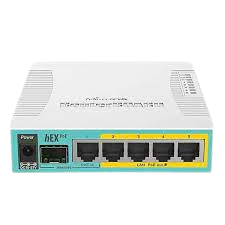
\includegraphics[width=0.5\linewidth]{P1/img/contoh.png}
		\caption{Step 1}
		\label{fig:gambar1}
	\end{figure}

	% poin 2
	\item Berikan IP address pada interface ether2 dan ether 4 yang dapat dibuat pada tab IP > Addresses. Berikan IP address sesuai dengan cara pengaturan IP address yang benar. Berikan IP
	address yang berbeda dengan contoh di modul.
	\begin{figure}[H]
		\centering
		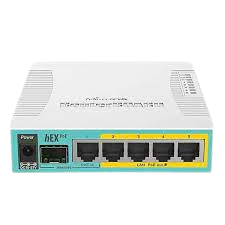
\includegraphics[width=0.5\linewidth]{P1/img/contoh.png}
		\caption{Step 2}
		\label{fig:gambar2}
	\end{figure}

	% poin 3.1
	\item Lakukan routing statis. Buka pada tab IP > Routes, lalu tambahkan jaringan.
	\begin{figure}[H]
		\centering
		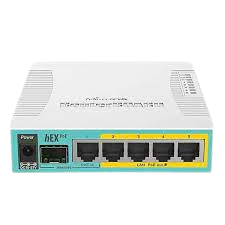
\includegraphics[width=0.5\linewidth]{P1/img/contoh.png}
		\caption{Step 3.1}
		\label{fig:gambar3}
	\end{figure}

	% poin 3.2
	Masukkan alamat jaringan yang ingin dituju, melalui alamat Gateway pada router 2
	
	\begin{figure}[H]
		\centering
		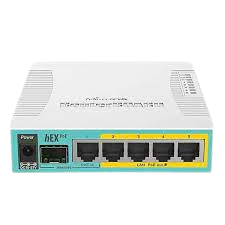
\includegraphics[width=0.5\linewidth]{P1/img/contoh.png}
		\caption{Step 3.2}
		\label{fig:gambar4}
	\end{figure}

\end{enumerate}

%Langkah untuk konfigurasi Router 2
\begin{center} 
	\textbf{Konfigurasi Router 2}
\end{center}

\begin{enumerate}
	% poin 1
	\item Buka WinBox dan lakukan koneksi ke Router 2

	% poin 2
	\item Berikan IP address pada interface ether2 dan ether 4 yang dapat dibuat pada tab IP > Addresses. Berikan IP address sesuai dengan cara pengaturan IP address yang benar. Berikan IP
	address yang berbeda dengan contoh di modul.
	\begin{figure}[H]
		\centering
		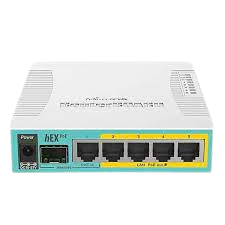
\includegraphics[width=0.5\linewidth]{P1/img/contoh.png}
		\caption{Step 2}
		\label{fig:gambar6}
	\end{figure}

	% poin 3
	\item Lakukan routing statis. Buka pada tab IP > Routes, lalu tambahkan jaringan. Masukkan alamat
	jaringan yang ingin dituju, melalui alamat Gateway pada router 1
	\begin{figure}[H]
		\centering
		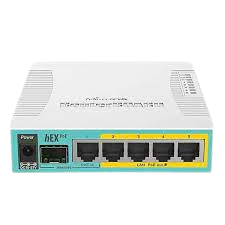
\includegraphics[width=0.5\linewidth]{P1/img/contoh.png}
		\caption{Step 3}
		\label{fig:gambar7}
	\end{figure}

\end{enumerate}

%Langkah untuk Mengecek keberhasilan konfigurasi
\begin{center} 
	\textbf{Mengecek keberhasilan konfigurasi}
\end{center}

\begin{enumerate}
	% poin 1
	\item Lakukan tes ping ke Router 2 melalui PC 1
	\begin{figure}[H]
		\centering
		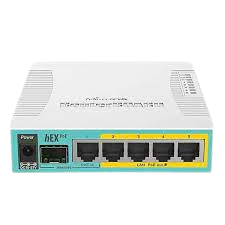
\includegraphics[width=0.5\linewidth]{P1/img/contoh.png}
		\caption{Step 1}
		\label{fig:gambar8}
	\end{figure}

	% poin 2
	\item Lakukan tes ping ke Router 1 melalui PC 2
	\begin{figure}[H]
		\centering
		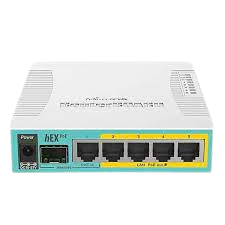
\includegraphics[width=0.5\linewidth]{P1/img/contoh.png}
		\caption{Step 2}
		\label{fig:gambar9}
	\end{figure}

\end{enumerate}

\subsection{Routing Dinamis}
Pada routing dinamis, terdapat setidaknya 3 jenis, yaitu :
\begin{enumerate}
	\item Routing Information Protocol (RIP) RIP adalah salah satu protokol routing dinamis yang menggunakan metrik hop count (jumlah hop) untuk menentukan jalur terbaik. Metrik hop count mengukur jarak antara router pengirim dengan tujuan dalam jumlah hop (melalui berapa banyak router).
	\item Open Shortest Path First (OSPF) OSPF adalah protokol routing dinamis yang menggunakan
	algoritma Dijkstra untuk menentukan jalur terpendek. OSPF mengumpulkan informasi topologi
	dari semua router dalam jaringan dan menghitung jalur terbaik berdasarkan bobot (cost) setiap
	link.
	Border Gateway Protocol (BGP) BGP adalah protokol routing eksternal yang digunakan di Internet. BGP memungkinkan router di AS (Autonomous System) yang berbeda untuk berkomunikasi dan menukar informasi routing
\end{enumerate}

%Langkah untuk konfigurasi Router 1
\begin{center} 
	\textbf{Konfigurasi Router 1}
\end{center}

\begin{enumerate}
	% poin 1
	\item Buka WinBox dan lakukan koneksi ke Router 1

	% poin 2
	\item Berikan IP address pada interface ether2 dan ether 4 yang dapat dibuat pada tab IP > Addresses. Berikan IP address sesuai dengan cara pengaturan IP address yang benar Berikan IP
	address yang berbeda dengan contoh di modul.
	\begin{figure}[H]
		\centering
		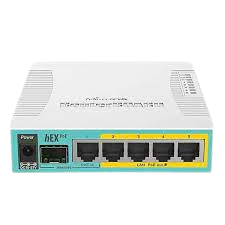
\includegraphics[width=0.5\linewidth]{P1/img/contoh.png}
		\caption{Step 2}
		\label{fig:gambar11}
	\end{figure}

	% poin 3.1
	\item Pada PC 1, lakukan routing dinamis. Buka tab Routing > RIP.
	\begin{figure}[H]
		\centering
		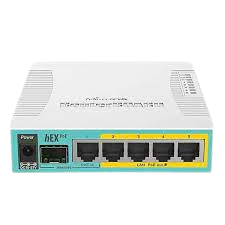
\includegraphics[width=0.5\linewidth]{P1/img/contoh.png}
		\caption{Step 3.1}
		\label{fig:gambar38}
	\end{figure}

	% poin 3.2
	Pada interface tambahkan interface baru kemudian ubah interface menjadi ether 4 dengan Receive dan Send pada v1.
	\begin{figure}[H]
		\centering
		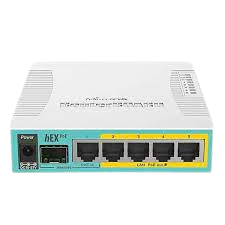
\includegraphics[width=0.5\linewidth]{P1/img/contoh.png}
		\caption{Step 3.2}
		\label{fig:gambar39}
	\end{figure}

	% poin 4
	\item Pada tab Network, tambahkan 2 network baru, yaitu network yang antara PC1 dengan Router
	1 dan network antara Router 1 dan Router 2.	
	\begin{figure}[H]
		\centering
		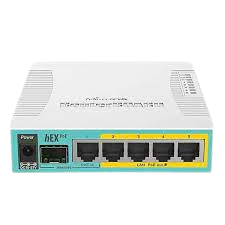
\includegraphics[width=0.5\linewidth]{P1/img/contoh.png}
		\caption{Step 4}
		\label{fig:gambar38}
	\end{figure}

	% poin 5
	\item Pada tab Neighbours, tambahkan alamat router yang dituju.
	\begin{figure}[H]
		\centering
		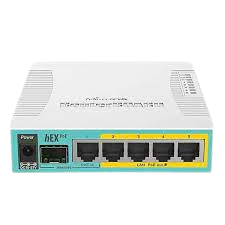
\includegraphics[width=0.5\linewidth]{P1/img/contoh.png}
		\caption{Step 5}
		\label{fig:gambar38}
	\end{figure}

\end{enumerate}

%Langkah untuk konfigurasi Router 2
\begin{center} 
	\textbf{Konfigurasi Router 2}
\end{center}

\begin{enumerate}
	% poin 1
	\item Buka WinBox dan lakukan koneksi ke Router 2
	
	% poin 2
	\item Berikan IP address pada interface ether2 dan ether 4 yang dapat dibuat pada tab IP > Addresses. Berikan IP address sesuai dengan cara pengaturan IP address yang benar. Berikan IP
	address yang berbeda dengan contoh di modul.
	\begin{figure}[H]
		\centering
		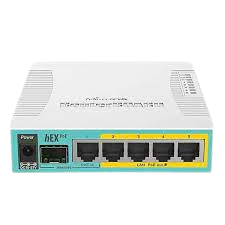
\includegraphics[width=0.5\linewidth]{P1/img/contoh.png}
		\caption{Step 2}
		\label{fig:gambar13}
	\end{figure}
	
	% poin 3
	\item Pada tab Network, tambahkan 2 network baru, yaitu network yang antara PC2 dengan Router
	2 dan network antara Router 1 dan Router 2.
	\begin{figure}[H]
		\centering
		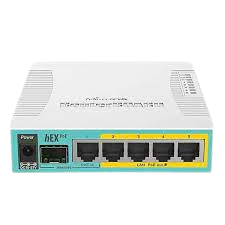
\includegraphics[width=0.5\linewidth]{P1/img/contoh.png}
		\caption{Step 3}
		\label{fig:gambar13}
	\end{figure}

	% poin 4
	\item Pada tab Neighbours, tambahkan alamat router yang dituju.
	\begin{figure}[H]
		\centering
		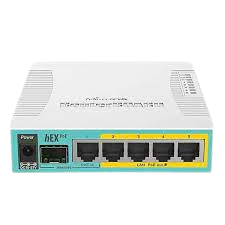
\includegraphics[width=0.5\linewidth]{P1/img/contoh.png}
		\caption{Step 4}
		\label{fig:gambar13}
	\end{figure}

\end{enumerate}

%Langkah untuk Mengecek keberhasilan konfigurasi
\begin{center} 
	\textbf{Mengecek keberhasilan konfigurasi}
\end{center}

\begin{enumerate}
	% poin 1
	\item Lakukan tes ping Router 2 dari PC 1
	\begin{figure}[H]
		\centering
		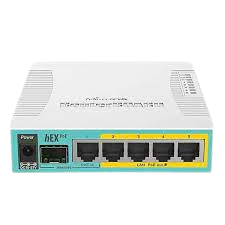
\includegraphics[width=0.5\linewidth]{P1/img/contoh.png}
		\caption{Step 1}
		\label{fig:gambar14}
	\end{figure}

	% poin 2
	\item Lakukan tes ping Router 1 dari PC 2
	\begin{figure}[H]
		\centering
		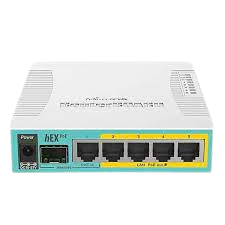
\includegraphics[width=0.5\linewidth]{P1/img/contoh.png}
		\caption{Step 2}
		\label{fig:gambar15}
	\end{figure}

\end{enumerate}

\section{Hasil Percobaan}
Hasil dari percobaan yang sudah kamu buat
%===========================================================%

\section{Kesimpulan}
simpulkan
%===========================================================%

\section{Lampiran}

\subsection{Tugas Pendahuluan}
\begin{enumerate}
	\item Buatlah topologi jaringan percobaan 1 dan 2!
	\begin{itemize}
		\item Topologi jaringan percobaan 1
		\begin{figure}[H]
		\centering
		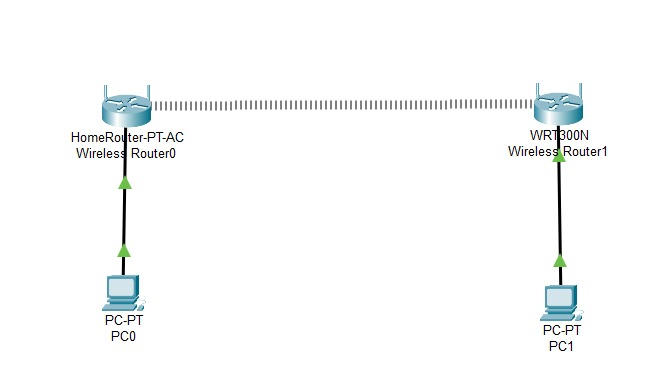
\includegraphics[width=0.7\linewidth]{P1/img/topologi1.jpg}
		\caption{Topologi Jaringan Percobaan 1}
		\label{fig:gambar31}
	\end{figure}


	\end{itemize}
	\begin{itemize}
		\item Topologi jaringan percobaan 2
		\begin{figure}[H]
			\centering
			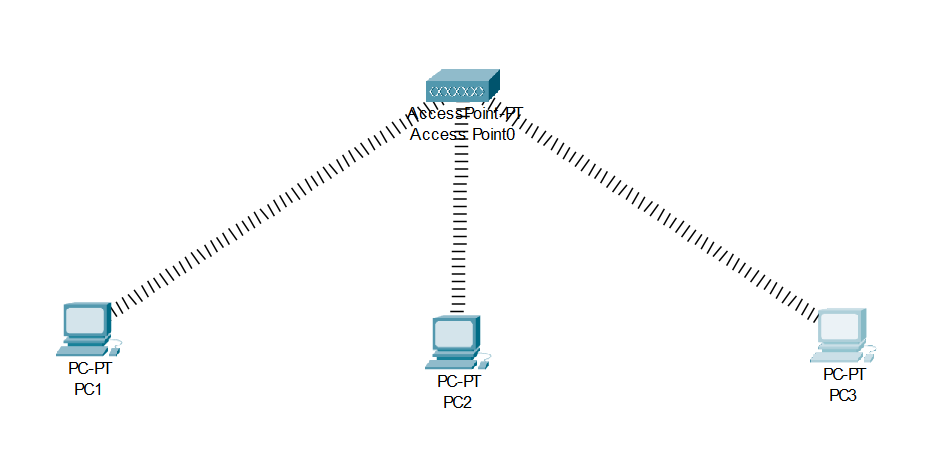
\includegraphics[width=0.7\linewidth]{P1/img/topologi2.png}
			\caption{Topologi Jaringan Percobaan 2}
			\label{fig:gambar32}
		\end{figure}
	\end{itemize}

	\item Perbedaan Point-to-Point, Point-to-Multipoint, dan Wireless Bridging
	\begin{itemize}
		\item Point-to-Point
		\begin{itemize}
			\item Point to point adalah metode pendistribusian akses internet yang hanya melibatkan 2 site saja.
			\item Hanya terdapat 1 radio station yang terkoneksi ke access point.
			\item Topologi PTP umumnya dipakai oleh ISP untuk mendistribusikan akses internet dari POP. 
			\item Kelebihan PTP adalah jaringan lebih stabil karena access point hanya akan memancarkan signalnya ke satu station saja, sehingga throughput yang dihasilkan akan maksimal. 
			\item Antena yang dipakai biasanya antena yang memiliki sudut pancaran 45-180 derajat (antena sectoral) atau 360 derajat (antena omni).
		\end{itemize}

		\item Point-to-Multipoint
		\begin{itemize}
			\item Menghubungkan satu access point ke beberapa station sekaligus
			\item PTMP biasanya dipakai untuk menekan biaya, karena hanya dengan satu radio access point saja sudah bisa mengkoneksikan beberapa radio station sekaligus. 
			\item Antena yang dipakai biasanya antena yang memiliki sudut pancaran 45-180 derajat (antena sectoral).
		\end{itemize}

		\item Wireless Bridging
		\begin{itemize}
			\item teknologi yang menghubungkan dua jaringan wireless yang berbeda, sehingga memungkinkan perangkat yang terhubung ke salah satu jaringan untuk dapat mengakses jaringan lainnya tanpa menggunakan kabel
			\item Wireless bridging dapat menghubungkan lebih dari 200 perangkat nirkabel secara bersamaan. 
			\item Fungsi Bridge juga mampu memindahkan data melalui intermediate network dengan tipe protokol sama sekali berbeda. 
			\item Bridge nirkabel memiliki fungsi yang lebih rumit dan berat ketimbang dua jenis Bridge yang sebelumnya.
		\end{itemize}
		
	\end{itemize}

	\item Follow IG Lab MIOT
	\begin{figure}[H]
		\centering
		\begin{subfigure}{0.3\linewidth}
			\centering
			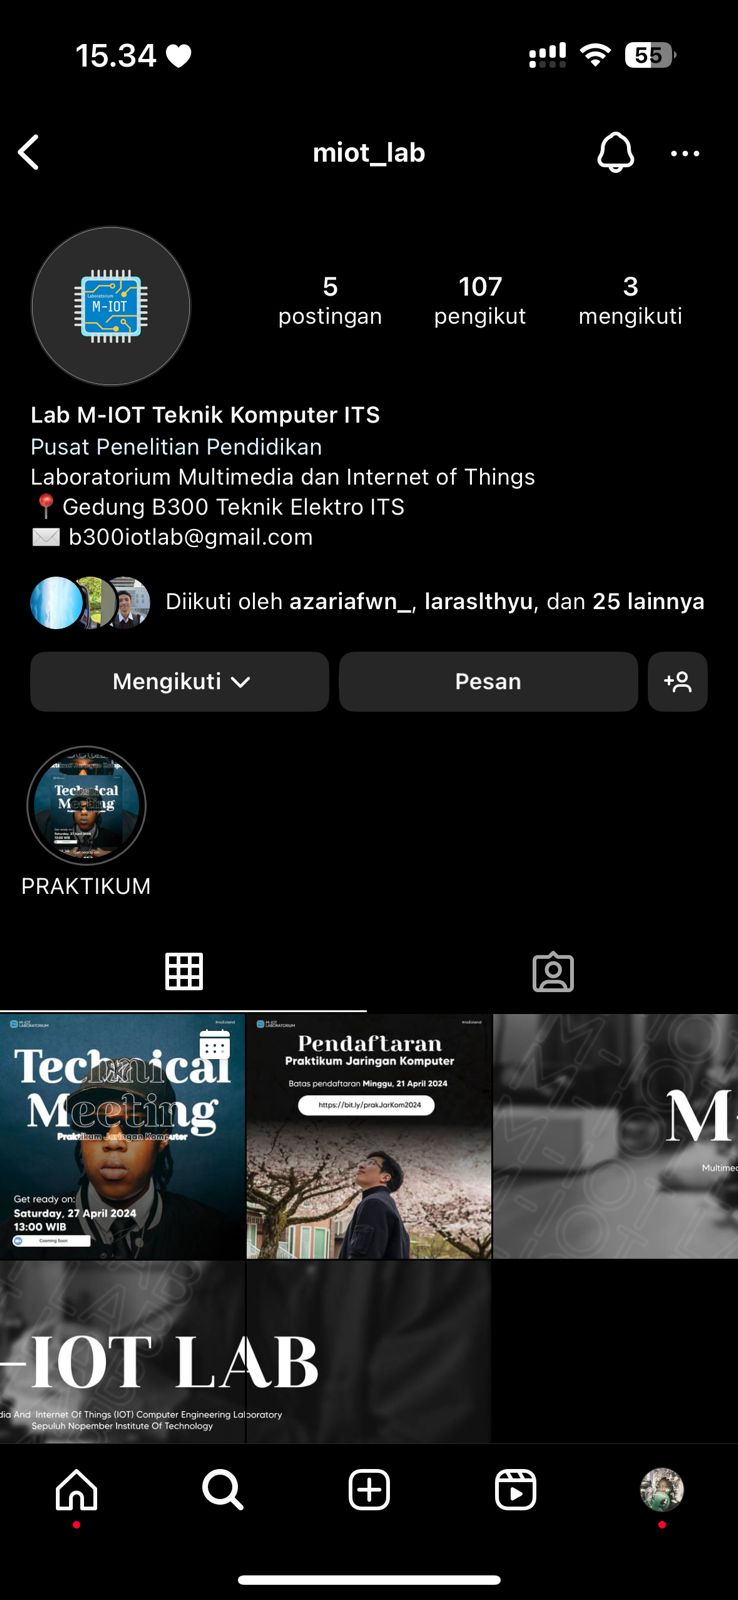
\includegraphics[width=\linewidth]{P1/img/vanfollow.jpg}
			\caption{Bukti Vania follow}
			\label{fig:gambar34}
		\end{subfigure}
		\begin{subfigure}{0.3\linewidth}
			\centering
			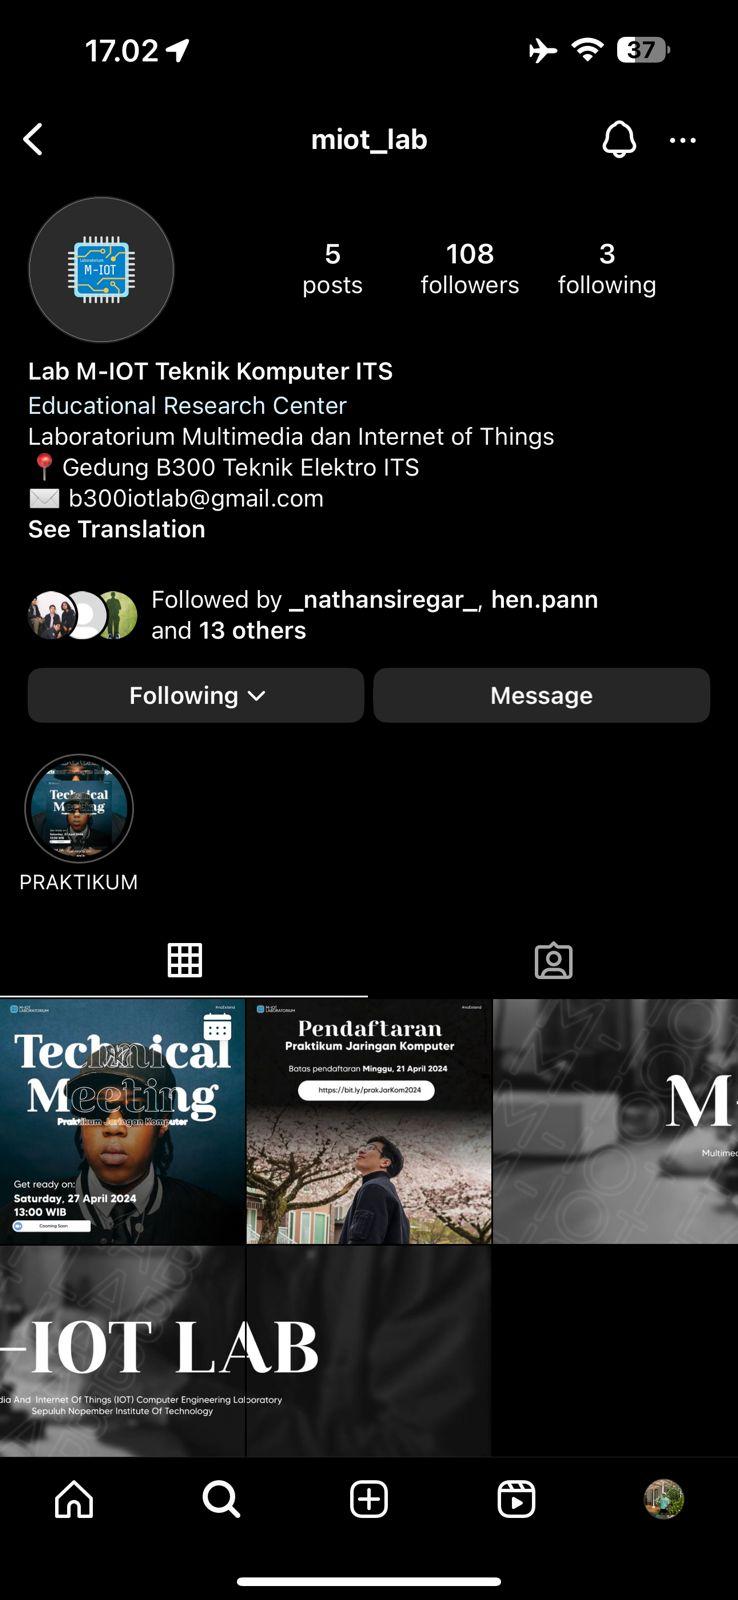
\includegraphics[width=\linewidth]{P1/img/cedfollow.jpg}
			\caption{Bukti Cedric follow}
			\label{fig:gambar35}
		\end{subfigure}
		\begin{subfigure}{0.3\linewidth}
			\centering
			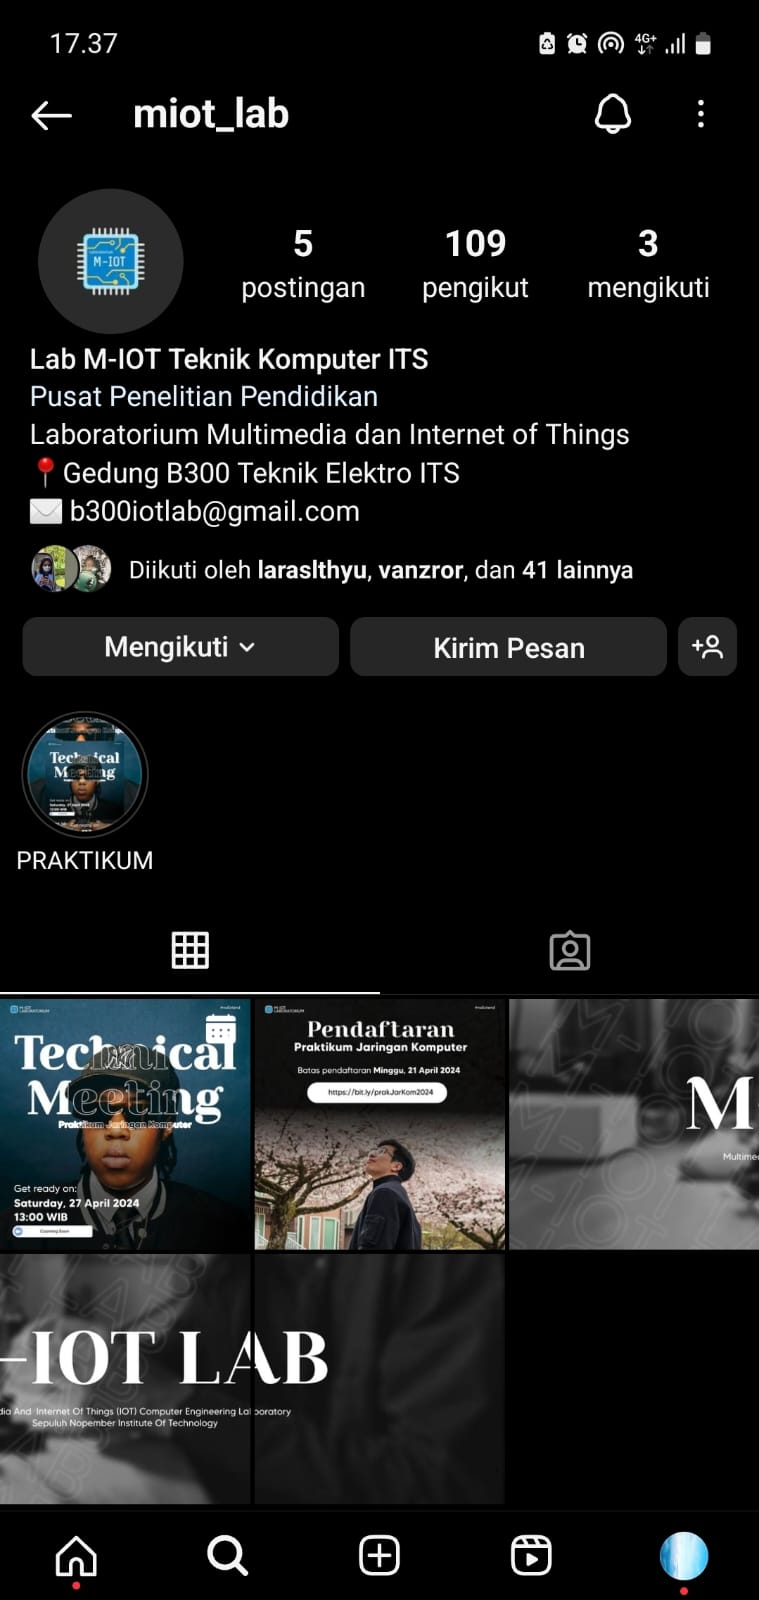
\includegraphics[width=\linewidth]{P1/img/zafafollow.jpg}
			\caption{Bukti Azaria follow}
			\label{fig:gambar36}
		\end{subfigure}
		\begin{subfigure}{0.8\linewidth}
			\centering
			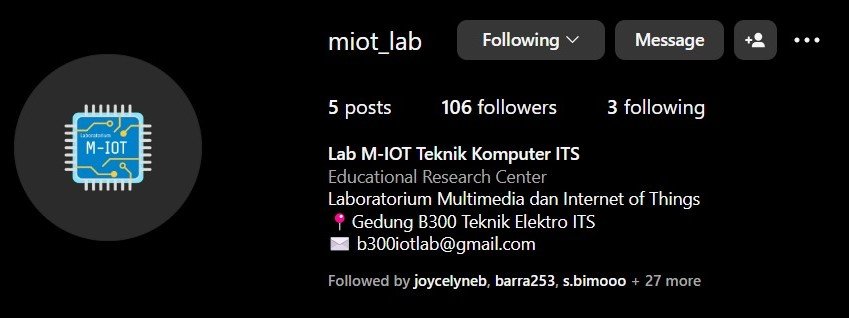
\includegraphics[width=\linewidth]{P1/img/larasfollow.jpg}
			\caption{Bukti Laras follow}
			\label{fig:gambar37}
		\end{subfigure}
		\caption{Bukti follow IG Lab MIOT}
		\label{fig:dua_gambar}
	\end{figure}
	
\end{enumerate}
\subsection{Dokumentasi saat Praktikum}

\end{document}

